%%%%%%%%%%%%%%%%%%%%%%%%%%%%%%%%%%%%%%%%%
% Beamer Presentation
% LaTeX Template
% Version 1.0 (10/11/12)
%
% This template has been downloaded from:
% http://www.LaTeXTemplates.com
%
% License:
% CC BY-NC-SA 3.0 (http://creativecommons.org/licenses/by-nc-sa/3.0/)
%
%%%%%%%%%%%%%%%%%%%%%%%%%%%%%%%%%%%%%%%%%

%----------------------------------------------------------------------------------------
%	PACKAGES AND THEMES
%----------------------------------------------------------------------------------------

\documentclass[14pt]{beamer}

\mode<presentation> {

% The Beamer class comes with a number of default slide themes
% which change the colors and layouts of slides. Below this is a list
% of all the themes, uncomment each in turn to see what they look like.

%\usetheme{default}
%\usetheme{AnnArbor}
%\usetheme{Antibes}
%\usetheme{Bergen}
%\usetheme{Berkeley}
%\usetheme{Berlin}
%\usetheme{Boadilla}
%\usetheme{CambridgeUS}
%\usetheme{Copenhagen}
%\usetheme{Darmstadt}
%\usetheme{Dresden}
%\usetheme{Frankfurt}
%\usetheme{Goettingen}
%\usetheme{Hannover}
%\usetheme{Ilmenau}
%\usetheme{JuanLesPins}
%\usetheme{Luebeck}
\usetheme{Madrid} %i was using this one
%\usetheme{Malmoe}
%\usetheme{Marburg}
%\usetheme{Montpellier}
%\usetheme{PaloAlto}
%\usetheme{Pittsburgh}
%\usetheme{Rochester}
%\usetheme{Singapore}
%\usetheme{Szeged}
%\usetheme{Warsaw}

% As well as themes, the Beamer class has a number of color themes
% for any slide theme. Uncomment each of these in turn to see how it
% changes the colors of your current slide theme.

%\usecolortheme{albatross}
%\usecolortheme{beaver}
%\usecolortheme{beetle}
%\usecolortheme{crane}
%\usecolortheme{dolphin}
%\usecolortheme{dove}
%\usecolortheme{fly}
%\usecolortheme{lily}
%\usecolortheme{orchid}
%\usecolortheme{rose}
%\usecolortheme{seagull}
%\usecolortheme{seahorse}
%\usecolortheme{whale}
%\usecolortheme{wolverine}

%\setbeamertemplate{footline} % To remove the footer line in all slides uncomment this line
%\setbeamertemplate{footline}[page number] % To replace the footer line in all slides with a simple slide count uncomment this line

%\setbeamertemplate{navigation symbols}{} % To remove the navigation symbols from the bottom of all slides uncomment this line
}

\usepackage{graphicx} % Allows including images
\usepackage{booktabs} % Allows the use of \toprule, \midrule and \bottomrule in tables
\usepackage{hyperref}
\usepackage{helvet}

%----------------------------------------------------------------------------------------
%	TITLE PAGE
%----------------------------------------------------------------------------------------

\title[Lab Intro]{Lab Intro and Computer Setup} % The short title appears at the bottom of every slide, the full title is only on the title page

\author{C. Ryan Campbell} % Your name
\institute[Duke] % Your institution as it will appear on the bottom of every slide, may be shorthand to save space
{
Duke University \\ % Your institution for the title page
\medskip
\textit{c.ryan.campbell@duke.edu} % Your email address
}
\date{31 Aug 2017} % Date, can be changed to a custom date

\begin{document}

\begin{frame}
\titlepage % Print the title page as the first slide
\end{frame}

\begin{frame}
\frametitle{Overview} % Table of contents slide, comment this block out to remove it
\tableofcontents % Throughout your presentation, if you choose to use \section{} and \subsection{} commands, these will automatically be printed on this slide as an overview of your presentation
\end{frame}

%----------------------------------------------------------------------------------------
%	PRESENTATION SLIDES
%----------------------------------------------------------------------------------------

%------------------------------------------------
\section{Intro} % Sections can be created in order to organize your presentation into discrete blocks, all sections and subsections are automatically printed in the table of contents as an overview of the talk
%------------------------------------------------

\subsection{Goals} % A subsection can be created just before a set of slides with a common theme to further break down your presentation into chunks

%------------------------------------------------
\begin{frame}
\frametitle{Today's Goals}
%what students should know/learn today
\begin{itemize}
	\item Get familiarized with course software
	\item Install software
	\item Produce a graph and save the code
%\sffamily
\end{itemize}
\end{frame}

%------------------------------------------------
\subsection{Computer Specs}

%------------------------------------------------
\begin{frame}
\frametitle{Computer Requirements}
\begin{itemize}
	\item Bring your computer to class
	\item Run some software locally
	\begin{itemize}
		\item How much empty storage do your laptops have?
	\end{itemize}
	\item Connect to cluster
\end{itemize}
%bring yours to every class
%run software from your computer
\end{frame}

%------------------------------------------------
\begin{frame}
\frametitle{Cluster Computing}
\begin{itemize}
	\item Duke Computing Cluster (DCC)
	\item SLURM workload manager
	\item Many cores, a lot of RAM, never shuts down
\end{itemize}
\end{frame}

%------------------------------------------------
\begin{frame}
\frametitle{Local vs. Cluster}
\begin{itemize}
	\item Which tasks are good for each of the following?
	\begin{itemize}
	\item<+-> RNAseq analysis 
	\item<+-> Statistical analysis 
	\item<+-> Sequence data `cleaning' 
	\item<+-> Producing plots 
	\end{itemize}
\end{itemize}
\end{frame}

%------------------------------------------------
\begin{frame}
\frametitle{Local vs. Cluster}
\begin{itemize}
	\item Which tasks are good for each of the following?
	\begin{itemize}
	\item RNAseq analysis (DCC)
	\item Statistical analysis (DCC/Local)
	\item Sequence data `cleaning' (DCC)
	\item Producing plots (Local)
	\end{itemize}
\end{itemize}
\end{frame}

%------------------------------------------------
\subsection{Tools}

%------------------------------------------------
\begin{frame}
\frametitle{Research Tools}
\begin{itemize}
	\item<1-> github
	\begin{itemize}
	\item<1-> Website for version control as well as script and code storage
	\end{itemize}

	\item<2-> R
	\begin{itemize}
	\item<2-> Statistical software, data visualization and analysis
	\end{itemize}
	
	\item<3-> kallisto/tophat/cufflinks
	\begin{itemize}
	\item<3-> Various RNAseq analysis packages
	\end{itemize}
	
\end{itemize}
\end{frame}

%------------------------------------------------
\begin{frame}
\frametitle{Programming Languages}
\begin{itemize}
	\item R
	\begin{itemize}
		\item free statistical software
	\end{itemize}
	\item bin/bash
	\begin{itemize}
		\item unix language, automate many tasks, interact with cluster computers
	\end{itemize}
\end{itemize}
\end{frame}

%------------------------------------------------
\begin{frame}
\frametitle{Software}
\begin{itemize}
	\item<1-> R - R-Studio
	\item<2-> github - SourceTree
	\item<3-> data analysis software - 
	\begin{itemize}
		\item fastqc
		\item trimmomatic
		\item kallisto/tophat/cufflinks
		\begin{itemize}
			\item we'll worry about these later
		\end{itemize}
	\end{itemize}
\end{itemize}
\end{frame}

%------------------------------------------------
\section{Lab}

%------------------------------------------------
\subsection{github}

%------------------------------------------------
\begin{frame}
\frametitle{github}
\begin{itemize}
	\item Software version control
	\item Shared and collaborative script editing
	\item Free!
	\item SourceTree
\end{itemize}
\end{frame}

%------------------------------------------------
\begin{frame}
\frametitle{github}
\begin{itemize}
	\item Create a github account
	\item \href{https://github.com/}{github.com}
	\item Create a repository for this course
	\item \href{https://guides.github.com/activities/hello-world/}{github Repo Tutorial}
	\item Make a repo for this course instead of ``hello-world''
\end{itemize}
\end{frame}

%------------------------------------------------
\begin{frame}
\frametitle{SourceTree}
\begin{itemize}
	\item Download and install SourceTree
	\item \href{https://www.sourcetreeapp.com/}{SourceTree Webpage}
	\item If you already have your own software, feel free to continue to use that
	\item Clone your repository onto your own computer
\end{itemize}
\end{frame}

%------------------------------------------------
\begin{frame}
\frametitle{SourceTree - Log in}
\begin{itemize}
	\item Open SourceTree
	\item Under Preferences ``Add Account'' and log into your github
\end{itemize}
\end{frame}

%------------------------------------------------
\begin{frame}
\frametitle{SourceTree - Clone a repo}
\begin{itemize}
	\item Click ``+New Repository''
	\item Select ``Clone from URL''
	\item On your github repo page click the green button labeled ``Clone or download''
	\item Copy the link and clone
\end{itemize}
\end{frame}

%------------------------------------------------
\begin{frame}
\frametitle{SourceTree - Test it out}
\begin{itemize}
	\item add a folder ``LabIntro'' maybe
	\item make a text file
	\begin{itemize}
		\item WARNING - github handles .txt files well, .doc files not well, so use ``notepad++'' or ``Sublime'' or ``TextWrangler'' to edit the files
	\end{itemize}
	\item Test SourceTree by committing the changes to the master branch, etc
\end{itemize}
\end{frame}

%------------------------------------------------
\subsection{R (like a pirate)}

%------------------------------------------------
\begin{frame}
\frametitle{R}
\begin{itemize}
	\item Statistical analysis and visualization
	\item Shared and collaborative script editing
	\item Free!
\end{itemize}
\end{frame}

%------------------------------------------------
\begin{frame}
\frametitle{R and R-Studio}
\begin{itemize}
	\item Download and install R
	\item \href{https://cran.rstudio.com/}{R download}
	\item Download and install R-Studio
	\begin{itemize}
		\item Desktop and Open Source Version
	\end{itemize}
	\item \href{https://www.rstudio.com/products/rstudio/download/}{R-Studio download}
\end{itemize}
\end{frame}

%------------------------------------------------
\begin{frame}
\frametitle{R-Studio Test}
\begin{itemize}
	\item Download my .Rmd script and datafile from github
	\begin{itemize}
		\item hypoxia analysis Rmd
		\item hsap hypoxia gene exp FORCLASS diff
	\end{itemize}
	\item Save it to your repo
	\item Run it in R-Studio to produce the graph
\end{itemize}
\end{frame}

%------------------------------------------------
\begin{frame}
\frametitle{R-Studio Test}
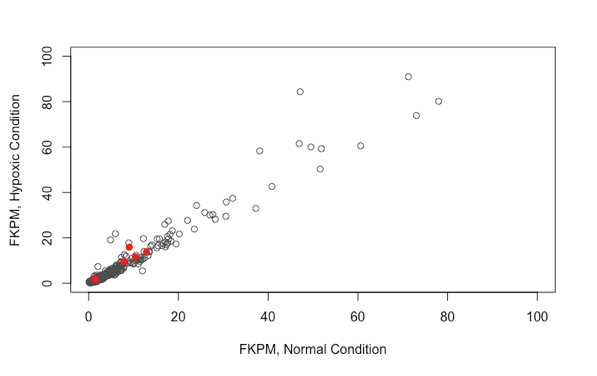
\includegraphics[width=0.8\linewidth]{images_20170831_rstudioplot.png}
\end{frame}

%------------------------------------------------
\begin{frame}
\frametitle{R-Studio Assignment}
\begin{itemize}
	\item Pick a different Gene Family
	\item Modify my code and plot the data
	\item Turn in -
	\begin{itemize}
		\item Your Plot
		\item A short paragraph about which gene family you picked an the results you saw
	\end{itemize}
\end{itemize}
\end{frame}

%------------------------------------------------
\begin{frame}
\frametitle{RNAseq Diff Files}
\begin{itemize}
	\item Output from a comparison across conditions
	\item Columns -
	\begin{itemize}
		\item gene family
		\item sample 1 and 2 - experimental condition of the sample
		\item status - were there non-zero values on both samples
		\item value 1 and 2 - relative amount of expression measured
		\item log fold change - difference between conditions, roughly
		\begin{itemize}
			\item negative numbers = decrease in expression from 1 to 2
		\end{itemize}
		\item test stat - test statistic
		\item p-value
		\item q-value
		\item significant - less than .05 p-val
	\end{itemize}
\end{itemize}
\end{frame}

%------------------------------------------------
\begin{frame}
\frametitle{Hypoxia Gene Families}
\begin{itemize}
	\item TOMM - Translocase of outer mitochondrial membrane
	\item TIMM - Translocase of inner mitochondrial membrane
	\item ZNF - Zinc Finger
	\item RAS - involved in transmitting signals within cells
	\item OR - Olfactory Receptors
	\item PK - Protein Kinases
	\item HK - Hexokinase
	\item NFK - Nuclear Factor Kappa
\end{itemize}
\end{frame}


%------------------------------------------------
\begin{frame}
\Huge{\centerline{The End}}
\end{frame}

%----------------------------------------------------------------------------------------

\end{document} 